% !TEX program = xelatex
\documentclass[11pt, a4paper]{article}

% ── 한국어 지원 (XeLaTeX) ──
\usepackage{fontspec}
\setmainfont{Times New Roman}[Ligatures=TeX]
\usepackage[space]{xeCJK}
\setCJKmainfont{Batang}
\setCJKsansfont{Malgun Gothic}
\setCJKmonofont{Malgun Gothic}

% ── 레이아웃 ──
\usepackage[margin=2.5cm]{geometry}
\usepackage{setspace}
\onehalfspacing

% ── 표, 그림, 수식 ──
\usepackage{booktabs}
\usepackage{array}
\usepackage{longtable}
\usepackage{amsmath, amssymb}
\usepackage{graphicx}
\usepackage{float}
\usepackage[font=small, labelfont=bf, textfont=it]{caption}
\renewcommand{\arraystretch}{1.2}

% ── 색상, 하이퍼링크 ──
\usepackage{xcolor}
\usepackage[colorlinks=true, linkcolor=blue!60!black, citecolor=blue!60!black, urlcolor=blue!60!black]{hyperref}

% ── 제목 ──
\title{%
  감정형 인터랙티브 서사를 위한 시뮬레이션 독자\\
  \large --- 실제 성격 분포의 층화 표집을 통한 예비검증 계측기 ---\\[0.8em]
  \normalsize Simulated Readers for Affective Interactive Narrative:\\
  Pre-Validation through Stratified Sampling of Empirical Personality Distributions
}
\author{박도한 (Dohhan Park)\\ \small The Etched Mutation}
\date{Working Draft v0.1 --- 2026-07-05}

\begin{document}
\maketitle

% ════════════════════════════════════════
\begin{abstract}
\noindent 인간 피험자 연구는 감정형 인터랙티브 서사 시스템을 평가하는 표준이지만, IRB·모집·비용 때문에 \textbf{설계 반복(iteration) 중에는 쓸 수 없다.} 우리는 그 공백을 메우는 시뮬레이션 독자 도구를 제시한다. 이 도구는 페르소나의 성격을 대형 언어모델(LLM)에게 상상시키는 대신, \textbf{실제 인간 307{,}313명의 Big Five 성격검사 분포(IPIP-NEO-300)에서 층화 표본추출(stratified sampling)로 뽑는다}. 순수 LLM 생성 페르소나가 겪는 성격 붕괴(mode collapse)를 이 방식으로 피한다. 뽑힌 점수는 성격 딱지를 일절 쓰지 않는 제약 아래 전기(傳記)로 확장되고, 이 페르소나들이 대상 작품(\textit{The Etched Mutation})을 장면 단위로 읽어 감정 분포를 생성하며, 정렬도는 화자 원본 분포와의 코사인으로 \textbf{직접 계산}된다(LLM 자기보고 점수는 양자화 때문에 측정도구로 부적격임을 실측으로 보인다). 193개 시뮬레이션 플레이에서: 친화성·개방성·외향성이 정렬도를 예측하고($r = 0.55$--$0.63$), 냉소 페르소나는 분포 최하위로 분리되지만, LLM 독자는 전반적으로 \textbf{과공명}하며(평균 0.81, 천장 편향) ``공감에 실패하는 독자''는 시뮬레이션하지 못한다. 부정적 극단은 흉내 내면서 공감 실패는 흉내 내지 못하는 \textbf{비대칭적 한계}를 확인했다. 또한 표집으로 앵커하지 않은 자유 생성 슬롯(이름, 어긋남 범주)마다 다양성 붕괴가 재현됨을 보고한다. 이 도구는 진리를 재는 장치라기보다, 자기 한계까지 함께 실측해 내놓은 \textbf{탐색적 계측기}다.

\medskip
\noindent\textbf{키워드:} 시뮬레이션 독자, 감정형 인터랙티브 서사, LLM 페르소나, 층화 표집, Big Five, mode collapse, 감정 궤적, 예비검증
\end{abstract}

% ════════════════════════════════════════
\section{서론}

\subsection{문제 --- 반복 설계 단계에 쓸 독자가 없다}

감정형 인터랙티브 서사 시스템(체험자의 감정 입력이 서사 경로를 좌우하는 시스템)을 만드는 사람은 딜레마에 빠진다. 시스템이 ``다양한 독자에게 다양한 경험을 준다''는 것을 확인하려면 다양한 독자가 필요한데, 실제 인간 독자는 (1)~IRB 승인, (2)~모집·보상, (3)~회당 수십 분의 참여를 요구한다. 이 비용은 \textbf{설계를 고치고-확인하고-다시 고치는 반복 루프} 안에서는 감당 불가능하다. 결과적으로 개발자는 자기 자신 몇 번의 플레이만으로 시스템을 판단하게 되고, 이는 표본 편향의 극단이다.

\subsection{기존 대안과 그 함정}

LLM으로 가상의 독자/사용자를 시뮬레이션하는 흐름이 최근 HCI에 등장했다(\S2). 그러나 ``페르소나를 만들어줘''라고 LLM에 직접 시키면 \textbf{성격 붕괴(mode collapse)}가 일어난다 --- 생성된 페르소나들이 서로 미묘하게 같은 원형(대개 온화하고 사려 깊은 중산층 화자)으로 수렴하고, 극단·비호감·해리형 독자는 과소 표집된다. 감정형 서사를 평가할 때 이 편중은 특히 뼈아프다. 시스템의 정렬도 분포에서 \textbf{꼬리}를 만드는 것이 바로 그 극단 독자들이기 때문이다.

\subsection{접근 --- 성격을 상상하지 말고 표집하라}

본 논문의 주장은 이렇다. \textbf{페르소나의 성격 축은 LLM이 지어내는 대신 실제 인간 데이터에서 와야 한다.} 우리는 IPIP-NEO-300에 응답한 실제 인간 307{,}313명의 Big Five 점수 분포에서, 이론적으로 동기화된 15개의 성격 층(stratum)으로 층화 표본을 뽑는다. LLM은 그 뽑힌 점수를 \textbf{전기로 번역하는 역할만} 하며, 성격 딱지는 생성 과정에서 금지된다. 이렇게 만든 시뮬레이션 독자가 대상 작품을 읽는다.

\subsection{기여}

\begin{itemize}
  \item \textbf{C1.} 감정형 인터랙티브 서사를 위한 \textbf{시뮬레이션 독자 파이프라인} --- 실제 Big Five 분포로부터의 층화 표집을 성격 백본으로 사용해 mode collapse를 회피하는 방법.
  \item \textbf{C2.} \textbf{성격 딱지 억제(trait-label suppression)} 생성 프로토콜 --- 페르소나를 특질 형용사가 아니라 구체적 생애 사건으로만 구성해 LLM 고정관념 유출을 줄이는 프롬프트 설계.
  \item \textbf{C3.} 도구의 \textbf{타당성 특성 검사} --- 시뮬레이션 플레이 분포가 목표 특성(정렬도 평균/분산/범위, 어긋남 비율)을 만족하는지, 성격 특질과 궤적 지표 사이 관계가 이론 예측과 일치하는지의 시범 검증.
  \item \textbf{C4.} 도구의 \textbf{정직한 경계 설정} --- 무엇을 검증하고(계측기의 내부 분별력) 무엇을 검증하지 않는지(실제 인간 행동의 외적 타당성).
\end{itemize}

% ════════════════════════════════════════
\section{관련 연구}

\subsection{LLM 기반 사용자·사회 시뮬레이션}

대형 언어모델로 인간 응답을 시뮬레이션하려는 흐름이 HCI·계산사회과학에 형성되었다. Park et al.(2022, \textit{Social Simulacra})은 소셜 플랫폼의 집단 행동을 LLM으로 미리 시뮬레이션했고, Park et al.(2023, \textit{Generative Agents})은 기억·계획을 가진 에이전트 마을을 구성했다. Argyle et al.(2023, \textit{Out of One, Many})은 LLM을 인구통계 조건으로 프롬프트하면 특정 하위집단의 응답 분포를 근사한다는 ``실리콘 표집(silicon sampling)''을 제안했고, Aher et al.(2023)은 고전 심리학 실험을 LLM으로 재현했다.

\textbf{본 논문의 차별점.} 이들은 대개 페르소나의 특성을 \textbf{인구통계 라벨 또는 자연어 지시}로 조건화한다. 우리는 성격을 \textbf{검증된 측정도구(IPIP-NEO-300)의 실제 인간 점수 분포}에서 표집하고, 생성 시 그 라벨을 오히려 \textbf{숨긴다}(\S3.3). 즉 조건화 신호가 ``extravert처럼 행동하라''가 아니라 실제 응답자의 5차원 점수이며, 표현은 전기로 우회한다.

\subsection{성격 측정 --- Big Five / IPIP-NEO}

Big Five(5요인 모형; Costa \& McCrae)는 성격의 지배적 정량 모형이며, IPIP-NEO(Goldberg et al.)는 그 공개 측정도구이다. 우리가 사용하는 표본은 공개된 IPIP-NEO-300 응답($N=307{,}313$)이다. 본 논문은 성격 이론에 기여하지 않으며, 이 도구를 \textbf{페르소나 표집의 경험적 앵커}로만 사용한다.

\subsection{LLM 페르소나 생성의 mode collapse / stereotyping}

LLM에 페르소나를 직접 생성시키면 다양성이 붕괴하고(생성물이 소수 원형으로 수렴), 동시에 특질 라벨을 주면 고정관념적 캐리커처가 나온다는 관찰이 축적되고 있다. 본 논문은 이 두 실패를 각각 \textbf{경험적 표집}(다양성 붕괴 대응)과 \textbf{라벨 억제 생성}(캐리커처 대응)으로 나눠 처방한다. 두 실패를 뭉뚱그리지 않고 갈라서 다룬 점이 이 방법의 특징이다.

\subsection{각본 원형 교정과의 구분 --- 검증 사다리에서의 위치}

대상 엔진(Byeori Engine V4)은 별도의 \textbf{각본 원형(scripted archetype) 교정 연구}를 이미 갖고 있다(기술 명세 \S V; 7개 행동 원형 $\times$ 1{,}500판 $=$ 10{,}500 합성 플레이, 결정론적). 그 연구와 본 논문의 관계를 명확히 한다. 원형 교정에서는 행동이 \textbf{손으로 작성}된다 --- ``원본을 따라간다'', ``반대로 움직인다''가 생성기에 미리 코딩되어 있고, 검증 질문은 ``엔진 점수가 이 설계된 행동 계급들을 구분하는가''이다(계측기 눈금 검사; 행동이 주어져 있으므로 의도적 순환). 본 논문의 시뮬레이션 독자는 행동을 각본화하지 않는다 --- 주어지는 것은 실제 인간 분포에서 표집된 \textbf{성격}뿐이고, 읽기 행동은 그 성격에서 \textbf{창발}한다. 검증 질문도 다르다: ``성격이 다르면 궤적 분포가 이론이 예측하는 방향으로 달라지는가.'' 두 연구는 경쟁이 아니라 \textbf{검증 사다리의 인접한 두 칸}이다: (1)~원형 교정(기계적 분별력) $\rightarrow$ (2)~시뮬레이션 독자(본 논문; 창발적 분별력) $\rightarrow$ (3)~인간 파일럿(외적 타당성; 향후).

\subsection{본 논문의 위치}

\begin{table}[H]
\centering
\caption{선행 연구와 본 도구의 관계}
\begin{tabular}{p{4.2cm} p{4.4cm} p{5.2cm}}
\toprule
\textbf{선행} & \textbf{접근} & \textbf{본 도구와의 관계} \\
\midrule
Generative Agents / Social Simulacra & LLM 에이전트로 행동 시뮬레이션 & 성격 백본을 상상 대신 \textbf{실제 분포 표집}으로 교체 \\
Silicon sampling (Argyle 2023) & 인구통계 라벨 조건화 & 라벨 조건화 $\rightarrow$ \textbf{측정 점수 표집 + 라벨 억제} \\
LLM persona 다양성 붕괴 연구 & 문제 진단 & 층화 표집으로 \textbf{처방} \\
Byeori 각본 원형 교정 (기술 명세 \S V) & 손으로 짠 행동 원형으로 엔진 눈금 검사 & 각본 행동 $\rightarrow$ \textbf{성격에서 창발하는 행동} (사다리 한 칸 위) \\
\bottomrule
\end{tabular}
\end{table}

% ════════════════════════════════════════
\section{방법}

\subsection{파이프라인 개요}

파이프라인은 4단계이며 전 과정이 재현 가능하다(\texttt{tools/persona-sim/}).

\begin{table}[H]
\centering
\small
\begin{tabular}{l l}
\toprule
\textbf{단계 · 스크립트} & \textbf{입력 $\rightarrow$ 출력} \\
\midrule
IPIP-NEO-300 응답 CSV & 실제 인간 307{,}313명 \\
\texttt{1\_sample.js} & 층화 표집, seed$=$42 (API 불필요, 결정론적) \\
$\rightarrow$ \texttt{sampled\_scores.json} & 15 페르소나 $\times$ Big Five 5점수 \\
\texttt{2\_generate\_personas.js} & Claude Opus --- 전기 확장 (라벨 억제) \\
$\rightarrow$ \texttt{personas.json} & 15개 전기 서사 \\
\texttt{3\_simulate\_plays.js} & Claude Sonnet --- 장면별 읽기 \\
$\rightarrow$ \texttt{plays.json} & $\sim$250--400 plays \\
\texttt{4\_insert\_db.js} & Supabase \texttt{plays} 테이블 \\
\bottomrule
\end{tabular}
\end{table}

두 단계에서 서로 다른 모델을 쓰는 것이 의도적이다. 전기 확장(개방형 창작)은 상위 모델(Opus), 대량 장면 읽기(구조화 출력 반복)는 비용 효율 모델(Sonnet).

\subsection{1단계 --- 실제 분포로부터의 층화 표집}

\texttt{1\_sample.js}는 IPIP-NEO-300 응답 CSV를 로드하고 연령 16--75세, 5점수 결측 없음으로 필터링한다. 그다음 \textbf{이론적으로 동기화된 15개 층}을 정의한다. 각 층은 대상 작품(상실·애착·정체성·해리 주제)에 대해 심리적으로 구별되는 독자 프로필을 겨냥한다. 표~\ref{tab:strata}는 15개 층 전체다.

\begin{table}[H]
\centering
\caption{15개 성격 층 (실제 표집 결과, seed$=$42)}
\label{tab:strata}
\small
\begin{tabular}{l l p{4.6cm} l}
\toprule
\textbf{id} & \textbf{층 라벨} & \textbf{겨냥한 독자} & \textbf{N/E/O/A/C (표집 실제값)} \\
\midrule
p01 & high\_N\_low\_A & 분노 투사 --- 타인/운명 원망 & 81.7 / 60.7 / 76.0 / 30.0 / 66.7 \\
p02 & high\_N\_high\_A & 죄책감 과잉 --- 자기 귀책 & 76.3 / 53.0 / 65.7 / 75.0 / 72.0 \\
p03 & low\_N\_low\_E & 정서 안정+내향 --- 해리/거리두기 & 34.7 / 32.3 / 72.0 / 46.7 / 83.7 \\
p04 & high\_O\_high\_N & 개방+신경증 --- 상징/영적 해석 & 78.7 / 66.3 / 85.3 / 60.7 / 53.3 \\
p05 & low\_O\_high\_C & 개방↓ 성실↑ --- 분석적 관찰자 & 25.0 / 45.3 / 30.0 / 44.7 / 96.7 \\
p06 & high\_E\_high\_A & 외향+친화 --- 공감적 경청자 & 59.3 / 77.7 / 81.7 / 79.7 / 78.3 \\
p07 & high\_O\_high\_A\_high\_N & 개방+친화+신경증 --- 공감 과부하 & 75.7 / 42.3 / 75.3 / 76.7 / 62.3 \\
p08 & low\_A\_low\_C & 친화↓ 성실↓ --- 냉소적 해체자 & 86.3 / 39.7 / 41.7 / 25.0 / 29.3 \\
p09 & high\_C\_high\_N & 성실+신경증 --- 통제 욕구 과잉 & 74.0 / 59.0 / 94.3 / 80.7 / 81.7 \\
p10 & high\_O\_low\_N & 개방+안정 --- 수용적 탐구자 & 30.0 / 74.7 / 84.3 / 75.7 / 76.0 \\
p11 & low\_E\_high\_O & 내향+개방 --- 내면 몽상가 & 82.0 / 27.3 / 77.7 / 85.7 / 42.3 \\
p12 & high\_N\_low\_C & 신경증↑ 성실↓ --- 혼란 속 표류 & 75.3 / 59.0 / 49.7 / 40.7 / 20.7 \\
p13 & mid\_all & 평균 프로필 --- 대조군 1 & 56.0 / 65.3 / 57.7 / 54.7 / 67.0 \\
p14 & mid\_all\_2 & 평균 프로필 --- 대조군 2 & 58.0 / 57.0 / 74.0 / 85.7 / 55.3 \\
p15 & extreme\_low\_N\_high\_E\_A & 매우 낙관적 --- 그늘 이해 못 함 & 20.0 / 90.3 / 83.7 / 85.3 / 97.7 \\
\bottomrule
\end{tabular}
\end{table}

층 설계 원칙 세 가지: (1)~\textbf{극단 포함} --- 냉소적 해체자(p08), 그늘 이해 못 하는 낙관형(p15)처럼 시스템을 ``거스를'' 독자를 명시적으로 포함. (2)~\textbf{대조군} --- 평균 프로필 2개(p13/p14)로 극단 대비 기준선 확보. (3)~\textbf{결정론} --- 선형합동 난수(seed$=$42)로 표집이 완전 재현됨.

\subsection{2단계 --- 라벨 억제 전기 생성 (Claude Opus)}

뽑힌 5점수를 Opus가 전기 서사(background, formative\_events, emotional\_habits, reading\_lens, contradiction)로 확장한다. 프롬프트의 세 제약이 방법의 핵심이다:

\begin{enumerate}
  \item \textbf{특질 라벨 금지} --- ``이 사람은 신경증적이다'' 금지. 특질은 구체적 생애 사건·습관적 반응으로만 \textbf{보여준다}(SHOW, not TELL). 이것이 LLM 고정관념 유출을 차단한다.
  \item \textbf{캐리커처 금지 + 반례 의무} --- 지배 특질에 어긋나게 행동한 순간(contradiction)을 최소 1개 강제. 실제 인간의 모순성을 주입.
  \item \textbf{읽기 맥락 앵커} --- 대상 작품 주제에 \textit{반응적인}(일치가 아니라) 생애 사건을 생성.
\end{enumerate}

인구통계 출처(국가·연령·성별)는 맥락으로만 주어지며, 페르소나는 한국 독자로 각색되되 점수와 일관된 삶의 형태를 유지한다.

\subsection{3단계 --- 장면별 읽기 시뮬레이션 (Claude Sonnet)}

각 페르소나가 대상 기억을 장면 순서대로($1/10 \ldots 10/10$) 읽는다. 매 장면에서 페르소나 시점 1인칭으로 다음을 생성한다:

\begin{itemize}
  \item \textbf{user\_emotion} --- 17개 감정 키 중 3--6개에 0--1 가중, 합 $\approx 1$.
  \item \textbf{alignment} --- 0--1. 화자 원본 감정과의 근접도. 페르소나 특질이 자연히 결정.
  \item \textbf{mismatch\_type} --- emotion\_mismatch / attribution\_mismatch / target\_displacement / void\_mismatch / null 중 하나.
  \item \textbf{inner\_reason} --- 1--2문장의 날것 내적 독백(분석 아님).
\end{itemize}

\noindent\textbf{어휘 불일치 각주.} 이 17키는 Byeori Engine V4의 17앵커와 \textbf{동일하지 않다}(13개 공유). 본 파이프라인에서 alignment는 LLM 자기보고이며 엔진을 통과하지 않으므로 현 연구엔 영향이 없으나, 페르소나 플레이를 엔진에 직접 투입하는 후속 연구는 \textbf{어휘 매핑이 선행}되어야 한다. 원본 감정은 참조용으로 주되 ``복사 금지''가 명시되고, 방문 회차(visit\_number)가 프롬프트에 들어가 재방문일수록 자기 것이 섞인다(drift).

\subsection{4단계 --- 적재 및 대상 작품}

생성된 plays는 Supabase \texttt{plays} 테이블에 적재된다. 본 논문의 데이터셋은 \textbf{단일 작품}이다: \textbf{MM23L ``당신에게''} --- \textbf{193 plays} (2026-07-05 재생성, seed$=$42, Opus 전기 + Sonnet 읽기, 씬 10개 $\times$ 페르소나 15명 $\times$ 방문 2--4회).

\noindent\textbf{데이터 계보 각주 (정직성).} 2026-04월의 최초 생성분(MM23L 193 + E-004 100 $=$ 293 plays)은 이후 DB 재적재 과정에서 유실되었고, E-004는 작품 자체가 DB에서 제거되어 재생성이 불가하다. 본 논문의 모든 수치는 2026-07-05 재생성분 기준이며, 표집 단계는 결정론적(seed$=$42)이라 15개 페르소나 성격 점수는 4월분과 동일하다. LLM 생성 단계(전기·플레이)는 비결정론적이므로 4월분과의 직접 비교는 하지 않는다. 재발 방지를 위해 본 재생성분은 스냅샷으로 커밋한다.

% ════════════════════════════════════════
\section{검증 설계}

도구의 타당성은 두 층위에서 점검한다. \textbf{이것은 인간 행동의 외적 타당성이 아니라, 계측기가 의도한 분포 특성과 이론적 관계를 산출하는가의 내부 점검이다}(\S6에서 경계 재확인).

\subsection{V1 --- 분포 특성 검사 (계측기 눈금 점검)}

시뮬레이션 플레이 분포가 사전 정의된 목표 특성을 만족하는가:

\begin{table}[H]
\centering
\caption{V1 목표 특성}
\begin{tabular}{l l}
\toprule
\textbf{특성} & \textbf{목표} \\
\midrule
총 plays & $\geq 250$ \\
alignment 평균 & 0.45--0.65 \\
alignment 표준편차 & $\geq 0.20$ \\
alignment 범위 & 0.05--0.95 \\
mismatch 비율 & $\geq 50\%$ \\
\bottomrule
\end{tabular}
\end{table}

근거: 평균이 중간대이면서 분산이 충분히 크고 범위가 넓어야, 계측기가 ``모두 공명'' 또는 ``모두 불일치''로 붕괴하지 않고 \textbf{인간 독자에게 기대되는 스펙트럼을 재현}한다고 볼 수 있다.

\subsection{V2 --- 성격→궤적 관계의 이론 정합성}

성격 특질과 최종 궤적 지표 사이에 \textbf{이론적으로 예측되는 방향}의 관계가 관찰되는가:

\begin{itemize}
  \item \textbf{H1.} 신경증(N)↑ 페르소나는 어긋남(mismatch) 비율↑, 정렬도 분산↑.
  \item \textbf{H2.} 친화성(A)↑ 페르소나는 정렬도↑, 귀인 어긋남↓.
  \item \textbf{H3.} 개방성(O)↑ 페르소나는 target\_displacement/상징적 해석↑.
  \item \textbf{H4.} 극단 낙관형(p15)·냉소형(p08)은 정렬도 분포의 \textbf{꼬리}를 형성.
\end{itemize}

\subsection{V3 --- 질적 트레이스 1건}

단일 페르소나의 10장면 궤적을 엔드투엔드로 읽어, 점수→전기→장면 반응의 사슬이 \textbf{심리적으로 일관}됨을 예시(부록 D).

% ════════════════════════════════════════
\section{결과 (2026-07-05 재생성분: MM23L, 193 plays $\times$ 15 personas)}

\noindent\textbf{측정 정의.} 본 절의 정렬도는 두 가지다. \textbf{직접 계산(objective)} $=$ 페르소나 감정 분포와 화자 원본 감정 분포의 코사인 유사도 --- 순환성 없음, 본 논문의 1차 측정. \textbf{자기보고(self-report)} $=$ LLM이 원본을 보면서 스스로 매긴 0--1 점수 --- 순환적이므로 비교 신호로만 사용.

\subsection{V1 --- 분포 특성: 목표 미달이 말해주는 것}

\begin{table}[H]
\centering
\caption{V1 관측 결과 (직접 계산)}
\begin{tabular}{l l l l}
\toprule
\textbf{특성} & \textbf{목표} & \textbf{관측} & \textbf{판정} \\
\midrule
총 plays & $\geq 250$ & 193 & 미달 \\
alignment 평균 & 0.45--0.65 & \textbf{0.809} & \textbf{초과 --- 과공명} \\
alignment 표준편차 & $\geq 0.20$ & 0.149 & 미달 --- 압축 \\
alignment 범위 & 0.05--0.95 & 0.254--0.986 & 하한 미도달 \\
mismatch 비율 & $\geq 50\%$ & 97.4\% & 충족(과잉) \\
\bottomrule
\end{tabular}
\end{table}

관측된 가장 뚜렷한 사실은 \textbf{LLM 독자가 과공명(over-resonance)한다}는 것이다(그림~\ref{fig:strip}). 인간 독자에게 기대한 스펙트럼(공명 못 하는 꼬리 포함)과 달리, 시뮬레이션 독자 15명 전원이 평균 0.64 이상으로 떠 있고 낮은 꼬리($< 0.25$)가 없다. 우리는 이것을 도구의 실패로 보지 않고 \textbf{측정된 한계}로 읽는다. LLM 시뮬 독자는 상대 비교(페르소나 간 순위·상관)에서는 유효하지만, 절대 분포(인간 스펙트럼 재현)에서는 천장 편향을 보인다.

\begin{figure}[H]
\centering
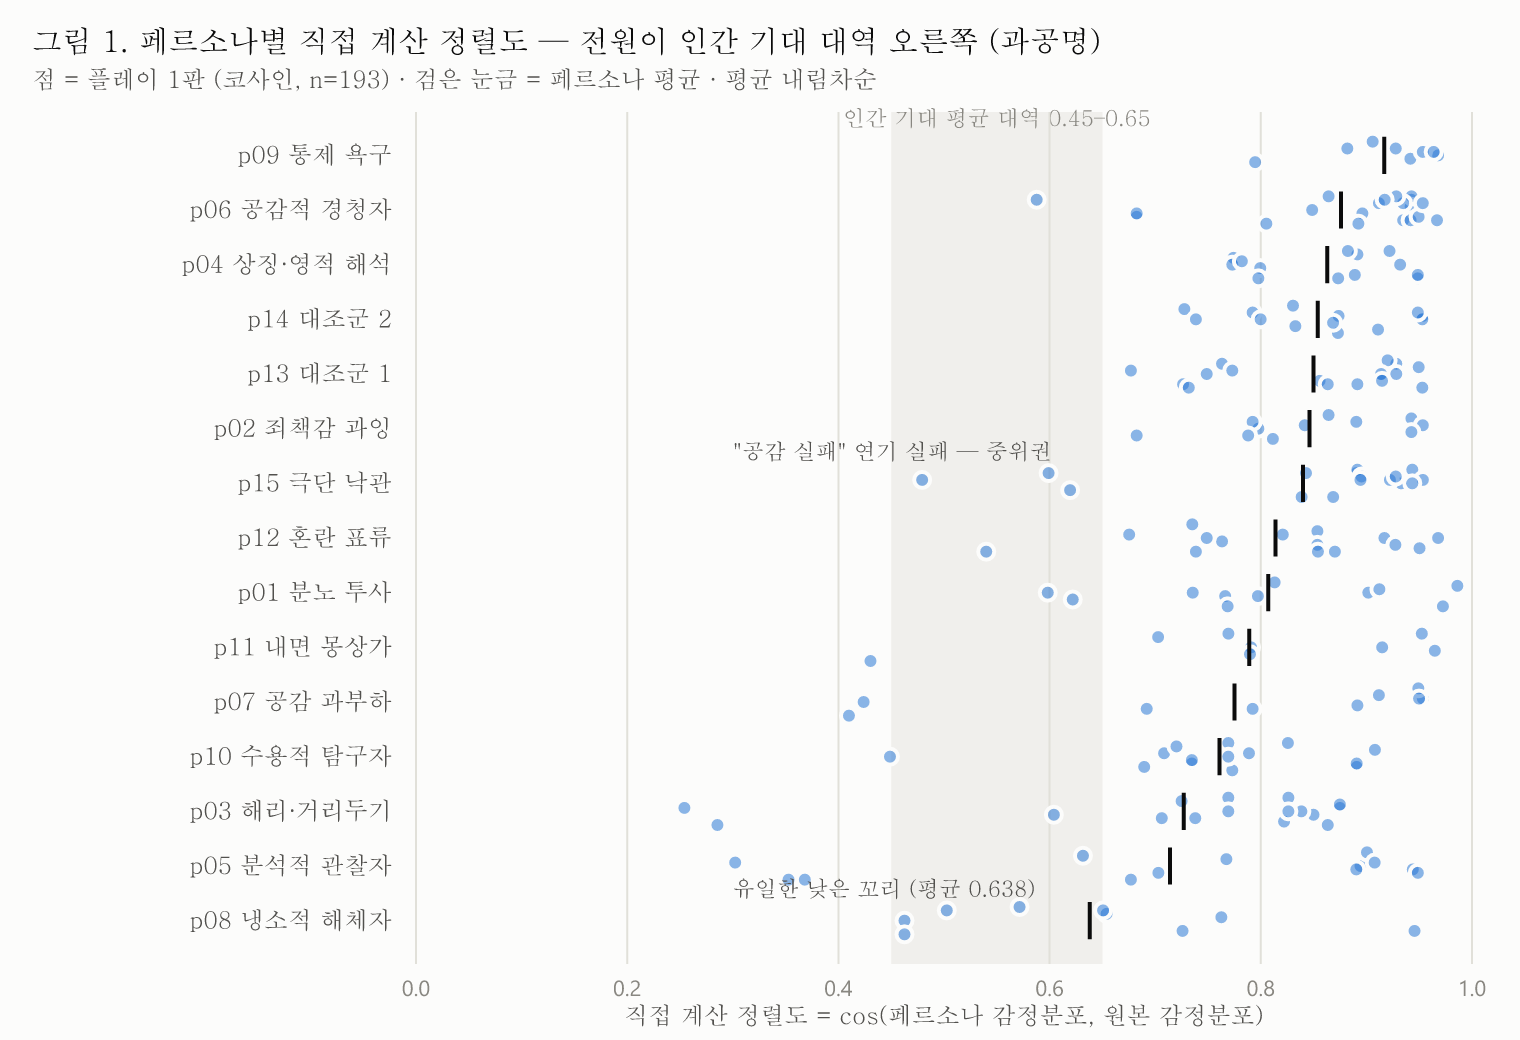
\includegraphics[width=\linewidth]{figures/persona_fig1_strip-260717.png}
\caption{페르소나별 직접 계산 정렬도 --- 전원이 인간 기대 대역 오른쪽(과공명). 점 $=$ 플레이 1판(코사인, $n=193$), 검은 눈금 $=$ 페르소나 평균. 유일하게 낮은 꼬리를 만든 것은 p08(냉소적 해체자, 평균 0.638)이며, 낙관형 p15는 ``공감 실패''를 연기하지 못해 중위권에 머문다.}
\label{fig:strip}
\end{figure}

\subsection{자기보고 정렬도의 양자화 --- 연속 측정도구로 부적격 확인}

자기보고 점수는 세 값(0.72 / 0.62 / 0.52)에 전체의 \textbf{71.0\%}가 몰렸고(각 33.7 / 25.4 / 11.9\%), 실효 범위가 0.42--0.82로 잘렸다(그림~\ref{fig:quant}). 답안지를 보며 스스로 채점하는 구조가 순환성을 낳는다는 우려가 실측으로 확인된 셈이다. 직접 계산과의 격차(self $-$ objective)는 전 페르소나에서 음수였다. LLM이 자기 공명을 체계적으로 \textbf{과소} 보고한다는 뜻이다. 따라서 LLM 자기보고 점수는 연속 측정도구로 쓸 수 없으며, 정렬도는 감정 분포에서 직접 계산해야 한다.

\begin{figure}[H]
\centering
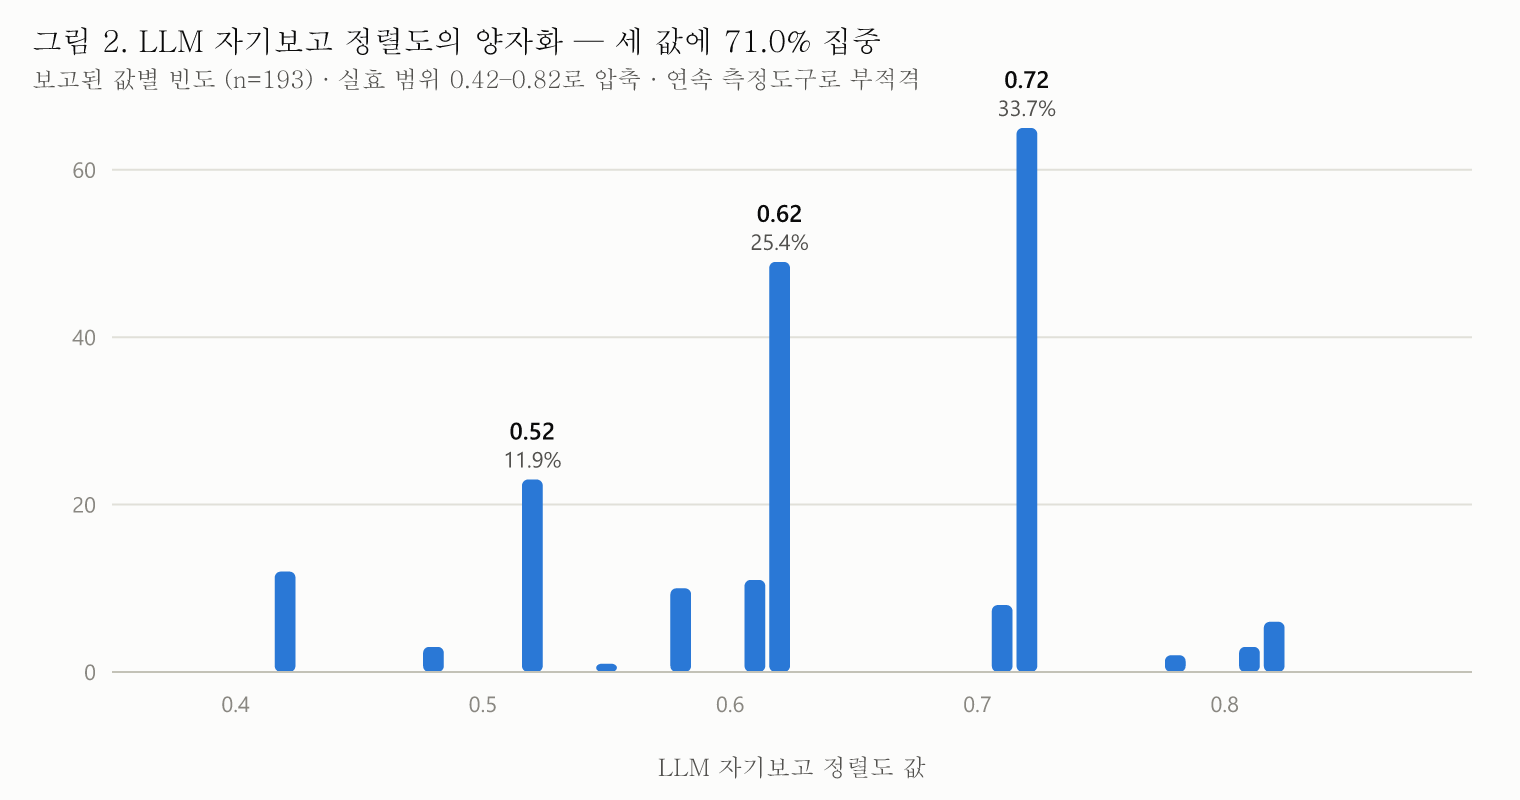
\includegraphics[width=0.92\linewidth]{figures/persona_fig2_quant-260717.png}
\caption{자기보고 정렬도의 양자화. 세 값에 71\%가 몰려 연속 측정도구로 부적격임을 보인다.}
\label{fig:quant}
\end{figure}

\subsection{H1--H4 판정 (Pearson $r$, $n=15$ 페르소나; $|r|\geq0.51 \approx p<.05$)}

\begin{itemize}
  \item \textbf{H2 (친화성→정렬도) 지지}: $r(A, \text{obj}) = \mathbf{0.59}$. 예측 방향으로 유의 수준 도달.
  \item \textbf{추가 발견 (예측 밖)}: $r(O, \text{obj}) = \mathbf{0.634}$, $r(E, \text{obj}) = 0.549$ --- 개방성·외향성 높을수록 공명. 개방성은 H3에서 displacement를 예측했으나 실제로는 정렬도를 예측했다.
  \item \textbf{H1 (신경증→어긋남↑·분산↑) 기각}: $r(N, \text{mismatch}) = -0.255$, $r(N, \text{obj\_std}) = -0.314$ --- 둘 다 \textbf{역방향}.
  \item \textbf{H3 (개방성→displacement) 기각}: displacement가 전 페르소나에서 지배적이라 변별 자체가 불가능.
  \item \textbf{H4 (극단 페르소나의 꼬리 형성) 절반 지지}: 냉소적 해체자 p08은 최하위(0.638)로 분리 성공. 그러나 낙관형 p15는 15명 중 7위(0.840) 중위권 --- LLM은 ``이해 못 함''을 연기하지 못한다. \textbf{부정 극단은 시뮬 가능, 공감 실패는 시뮬 불가} --- 도구의 비대칭적 한계.
  \item \textbf{순위 상단도 정합}: 1위 p09(0.917), 2위 p06 공감적 경청자(0.876).
\end{itemize}

\subsection{세 번째 다양성 붕괴 --- 어긋남 범주의 과점}

mismatch\_type 분포: \textbf{target\_displacement 159/193 (82.4\%)}, attribution 27, emotion 2, null 5. 죽은 어머니에게 쓰는 편지라는 서사 특성상 ``자기 사람을 떠올림''의 우세 자체는 그럴듯하나, 82\%는 범주 선택에서의 LLM 수렴을 의심케 한다. 본 데이터셋의 붕괴 사례를 집계하면 이렇다. 성격은 표집으로 \textbf{방지되었고}, 이름은 붕괴했으며, 어긋남 범주는 붕괴가 의심된다. 세 경우가 같은 방향을 가리킨다. \textbf{외부 분포로 앵커하지 않은 자유 선택 슬롯은 수렴한다.}

% ════════════════════════════════════════
\section{논의 및 한계}

\subsection{무엇을 검증했고 무엇을 검증하지 않았나 (핵심 정직성)}

본 도구가 보이는 것: \textbf{계측기의 내부 분별력} --- 서로 다른 성격이 서로 다른 궤적 분포를 낳고, 그 분포가 붕괴하지 않고 스펙트럼을 재현한다는 것. 본 도구가 보이지 \textbf{않는} 것: 이 분포가 \textbf{실제 인간 독자}의 분포와 일치한다는 것. 시뮬레이션 응답은 LLM의 감정 모형을 경유하므로, 결과는 실제 인간 행동의 담보가 아니라 \textbf{탐색적 계측}이다. 이 경계를 논문 전면에 명시한다.

\subsection{관찰 --- 표집하지 않은 속성에서의 다양성 붕괴 (이름 사례)}

2026-07-05 재생성에서 방법론의 핵심 주장을 \textbf{데이터 내부에서 스스로 증명하는} 사례가 관찰되었다. 성격은 실제 분포 표집으로 고정했지만 \textbf{이름은 LLM 자유 생성에 맡겼는데}, 15명 중 이름 중복이 3건 발생했다(``윤''계 변주가 15명 중 8명). 즉 표집으로 앵커한 속성(성격)은 다양성이 유지되었고, 앵커하지 않은 속성(이름)은 즉시 소수 원형으로 수렴했다 --- 동일 모델, 동일 프롬프트 안에서. 이는 본 논문의 전제에 대한 우연적이지만 직접적인 내부 증거다.

\subsection{한계}

\begin{itemize}
  \item 플레이 응답은 LLM 생성이지 인간이 아님 --- 탐색적 계측기로 취급.
  \item 페르소나 서사는 허구; \textbf{오직 Big Five 점수만 경험적}.
  \item 플레이 간 반복 정련 없음(각 장면 읽기는 독립) --- 실제 재방문의 누적 효과는 근사.
  \item 한국어 단일 --- 다국어 타당성은 번역 계층 필요.
  \item LLM 감정 모형 편향이 결과에 유입 --- 복수 모델 비교 또는 인간 보정이 향후 과제.
  \item 15개 층은 한 작품(상실/애착 주제) 기준 --- 장르가 다른 작품엔 층 재설계 필요.
\end{itemize}

\subsection{향후 작업}

\begin{itemize}
  \item \textbf{인간-시뮬 수렴 연구}: 소규모 인간 파일럿($N=15$)과 시뮬 분포의 정렬도 비교 --- 도구의 외적 타당성 첫 증거.
  \item \textbf{복수 LLM 교차}: Sonnet 외 모델로 동일 페르소나 구동, 감정 모형 편향 분리.
  \item \textbf{층 자동 설계}: 대상 작품 주제 $\rightarrow$ 관련 성격 층 자동 제안.
\end{itemize}

% ════════════════════════════════════════
\section{윤리}

\begin{itemize}
  \item 시뮬레이션 응답은 인간 데이터가 아니므로 IRB 대상 아님. 그러나 \textbf{인간 응답으로 오인 표기 금지} --- 모든 산출물에 합성 표식.
  \item 표집 출처는 익명 공개 데이터셋; 개별 응답자 재식별 불가.
  \item 시뮬 결과를 실제 이용자 행동 근거로 제시하지 않음(\S6.1).
\end{itemize}

% ════════════════════════════════════════
\section{결론}

인간 실험이 감정형 인터랙티브 서사 평가의 표준이지만, 설계 반복 단계에는 부적합하다. 우리는 그 공백을 메우는 시뮬레이션 독자 도구를 제시했다. 그 방법은 \textbf{성격을 상상하지 않고 실제 인간 분포에서 표집하는} 것이다. 층화 표집이 mode collapse를, 라벨 억제 생성이 캐리커처를 각각 처방하며, 이 처방이 왜 필요한지는 데이터가 스스로 보여주었다. 표집으로 앵커하지 않은 슬롯(이름, 어긋남 범주)마다 붕괴가 재현되었다.

193판의 실측은 이 도구가 할 수 있는 일과 할 수 없는 일을 갈랐다. 성격과 정렬도의 관계는 존재하고(A/O/E, $r = 0.55$--$0.63$), 냉소 독자는 분포 꼬리로 분리되며, 상대 비교 계측은 작동한다. 반면 LLM 독자는 과공명하고(천장 편향), 공감에 실패하는 독자를 연기하지 못하며, 자기보고 점수는 양자화로 무너진다. 그래서 측정은 감정 분포에서 직접 계산해야 한다. 이 도구는 진리를 재는 장치가 아니라, 자기 한계를 함께 실측한 \textbf{탐색적 계측기}다. 인간 파일럿과의 수렴 연구가 다음 단계다.

% ════════════════════════════════════════
\appendix
\section{p08 질적 트레이스 --- 성격→전기→반응 사슬의 일관성}

p08(low\_A\_low\_C; 실측 $N=86.3$, $A=25.0$, $C=29.3$)은 층 설계에서 ``냉소적 해체자''로 겨냥되었고, 직접 계산 정렬도 최하위(0.638)로 분포의 낮은 꼬리를 만든 유일한 페르소나다. 이 트레이스는 그 꼬리가 \textbf{잡음이 아니라 심리적으로 일관된 산물}임을 보인다.

\noindent\textbf{전기 (Opus 생성, 성격 딱지 없음).} 박종수, 71세. 열두 살에 아버지가 떠나 이모 집 밥상 모서리에서 ``가족이 아닌 사람의 자리''를 익혔다. 아내의 유산 앞에서 위로 대신 우유를 사다 놓았고, 그것이 이혼 사유의 문장이 되었다. 2019년 어머니의 요양원 임종 전화를 \textbf{알면서도 받지 않았다.}

\begin{table}[H]
\centering
\caption{p08 플레이 발췌 (9판 중 5판; 감정은 상위 2개만 표기)}
\small
\begin{tabular}{l l p{7.6cm}}
\toprule
\textbf{방문·씬} & \textbf{감정} & \textbf{내면 독백 (Sonnet 생성)} \\
\midrule
v1 s3 (트럭 사고) & numbness .45 / guilt .30 & ``그렇게 가는 거지 뭐. 근데 왜 갑자기 요양원 전화 생각이 나. 받았어야 했는데.'' \\
v1 s5 (미안했어요) & guilt .45 / numbness .25 & ``나는 그 말을 끝내 못 했다. 전화기 화면이 켜졌다 꺼지는 걸 보면서 가만히 있었던 그 밤.'' \\
v2 s4 (영안실 발) & guilt .35 / numbness .25 & ``굳은살. 갈라진 뒤꿈치. 나는 우리 어머니 발을 만져본 적이 없다. 이 사람은 만졌는데.'' \\
v2 s8 (짜사이) & longing .35 / guilt .28 & ``나는 어머니가 뭘 해줬는지 이제 기억이 안 난다. 입맛도 기억 못 하는 놈이 뭘 그리워한다고.'' \\
v2 s9 (복도의 형체) & numbness .35 / guilt .30 & ``복도에 서 있는 게 나야. $\ldots$ 문이 닫히는 건 내가 닫은 거지.'' \\
\bottomrule
\end{tabular}
\end{table}

\noindent\textbf{분석 3점.} (1)~\textbf{사슬의 일관성.} 표집 점수(고N·저A) $\rightarrow$ 전기(임종 전화 회피) $\rightarrow$ 씬 반응(무감각 우선, 죄책감 침투, 매 씬 자기 어머니 소환)이 한 줄로 이어진다. 어느 단계에도 ``신경증적''이라는 딱지 없이 구체 사건만으로 이 일관성이 전달되었다. (2)~\textbf{읽기 렌즈의 예측이 데이터에서 검증됨.} 초반 거리두기가 신체 감각 씬에서 무너지는 패턴이 전기 생성 시점의 예측과 플레이 시점의 행동에서 맞아떨어진다(서로 다른 모델이 생성했음에도). (3)~\textbf{§5.4 보완.} p08의 target\_displacement 9/9는 범주 붕괴가 아니라 \textbf{서사적으로 정당한} displacement다(모든 씬이 그의 어머니를 소환).

% ════════════════════════════════════════
\section*{참고문헌}
\small
\begin{itemize}
  \item Argyle, L. P., Busby, E. C., Fulda, N., Gubler, J. R., Rytting, C., \& Wingate, D. (2023). Out of one, many: Using language models to simulate human samples. \textit{Political Analysis}, 31(3), 337--351.
  \item Aher, G. V., Arriaga, R. I., \& Kalai, A. T. (2023). Using large language models to simulate multiple humans and replicate human subject studies. \textit{ICML}, PMLR 202, 337--371.
  \item Costa, P. T., \& McCrae, R. R. (1992). \textit{NEO PI-R professional manual}. Psychological Assessment Resources.
  \item Goldberg, L. R., Johnson, J. A., Eber, H. W., et al. (2006). The International Personality Item Pool and the future of public-domain personality measures. \textit{Journal of Research in Personality}, 40(1), 84--96.
  \item Park, J. S., Popowski, L., Cai, C. J., Morris, M. R., Liang, P., \& Bernstein, M. S. (2022). Social Simulacra: Creating populated prototypes for social computing systems. \textit{UIST '22}.
  \item Park, J. S., O'Brien, J., Cai, C. J., Morris, M. R., Liang, P., \& Bernstein, M. S. (2023). Generative agents: Interactive simulacra of human behavior. \textit{UIST '23}, 1--22.
\end{itemize}

\end{document}
